\documentclass[a4paper,twoside]{article}
\usepackage{blindtext}  
\usepackage{geometry}

% Chinese support
\usepackage[UTF8, scheme = plain]{ctex}

% Page margin layout
\geometry{left=2.3cm,right=2cm,top=2.5cm,bottom=2.0cm}


\usepackage{listings}
\usepackage{xcolor}
\usepackage{geometry}
\usepackage{amsmath}
\usepackage{float}
\usepackage{hyperref}

\usepackage{graphics}
\usepackage{graphicx}
\usepackage{subfigure}
\usepackage{epsfig}
\usepackage{float}

\usepackage{algorithm}
\usepackage[noend]{algpseudocode}

\usepackage{booktabs}
\usepackage{threeparttable}
\usepackage{longtable}
\usepackage{tikz}
\usepackage{multicol}
\usepackage{pgfplots}
\pgfplotsset{compat=1.9}
\pgfplotsset{
    myplotstyle/.style={
    legend style={draw=none, font=\small},
    legend cell align=left,
    legend pos=north east,
    ylabel style={align=center, font=\bfseries\boldmath},
    xlabel style={align=center, font=\bfseries\boldmath},
    x tick label style={font=\bfseries\boldmath},
    y tick label style={font=\bfseries\boldmath},
    scaled ticks=false,
    every axis plot/.append style={thick},
    },
}

% cite package, to clean up citations in the main text. Do not remove.
\usepackage{cite}

\usepackage{color,xcolor}

%% The amssymb package provides various useful mathematical symbols
\usepackage{amssymb}
%% The amsthm package provides extended theorem environments
\usepackage{amsthm}
\usepackage{amsfonts}
\usepackage{enumerate}
\usepackage{enumitem}
\usepackage{listings}
\usepackage{minted}


\usepackage{indentfirst}
\setlength{\parindent}{2em} % Make two letter space in the first paragraph
\usepackage{setspace}
\linespread{1.5} % Line spacing setting
\usepackage{siunitx}
\setlength{\parskip}{0.5em} % Paragraph spacing setting

% \usepackage[contents =22920202204622, scale = 10, color = black, angle = 50, opacity = .10]{background}

\renewcommand{\figurename}{图}
\renewcommand{\listingscaption}{代码}
\renewcommand{\tablename}{表格}
\renewcommand{\contentsname}{目录}
\floatname{algorithm}{算法}

\graphicspath{ {images/} }

%%%%%%%%%%%%%
\newcommand{\StudentNumber}{22920202204622}  % Fill your student number here
\newcommand{\StudentName}{熊恪峥}  % Replace your name here
\newcommand{\PaperTitle}{实验(一)}  % Change your paper title here
\newcommand{\PaperType}{实验报告} % Replace the type of your report here
\newcommand{\Date}{2023年3月21日}
\newcommand{\College}{信息学院}
\newcommand{\CourseName}{数据库}
%%%%%%%%%%%%%

%% Page header and footer setting
\usepackage{fancyhdr}
\usepackage{lastpage}
\pagestyle{fancy}
\fancyhf{}
% This requires the document to be twoside
\fancyhead[LO]{\texttt{\StudentName }}
\fancyhead[LE]{\texttt{\StudentNumber}}
\fancyhead[C]{\texttt{\PaperTitle }}
\fancyhead[R]{\texttt{第{\thepage}页,共\pageref*{LastPage}页}}


\title{\PaperTitle}
\author{\StudentName}
\date{\Date}

\algnewcommand\algorithmicinput{\textbf{Input:}}
\algnewcommand\algorithmicoutput{\textbf{Output:}}
\algnewcommand\Input{\item[\algorithmicinput]}%
\algnewcommand\Output{\item[\algorithmicoutput]}%

\usetikzlibrary{positioning, shapes.geometric}

\begin{document}
	
%%%%%%%%%%%%%%%%%%%%%%%%%%%%%%%%%%%%%%%%%%%%
\makeatletter % change default title style
\renewcommand*\maketitle{%
	\begin{center} 
		\bfseries  % title 
		{\LARGE \@title \par}  % LARGE typesetting
		\vskip 1em  %  margin 1em
		{\global\let\author\@empty}  % no author information
		{\global\let\date\@empty}  % no date
		\thispagestyle{empty}   %  empty page style
	\end{center}%
	\setcounter{footnote}{0}%
}
\makeatother
%%%%%%%%%%%%%%%%%%%%%%%%%%%%%%%%%%%%%%%%%%%%
	
	
\thispagestyle{empty}

\vspace*{1cm}

\begin{figure}[htb]
	\centering
	
\includegraphics[width=4.0cm]{logo.png}
\end{figure}

\vspace*{1cm}

\begin{center}
	\Huge{\textbf{\PaperType}}
	
	\Large{\PaperTitle}
\end{center}

\vspace*{1cm}

\begin{table}[H]
	\centering	
	\begin{Large}
		\renewcommand{\arraystretch}{1.5}
		\begin{tabular}{p{3cm} p{5cm}<{\centering}}
			姓\qquad 名 & \StudentName  \\
			\hline
			学\qquad号 & \StudentNumber \\
			\hline
			日\qquad期 & \Date  \\
			\hline
			学\qquad院 & \College  \\
			\hline
			课程名称 & \CourseName  \\
			\hline
		\end{tabular}
	\end{Large}
\end{table}

\newpage

\title{
	\Large{\textcolor{black}{\PaperTitle}}
}
	
	
\maketitle
	
\tableofcontents
 
\newpage
\setcounter{page}{1}

\begin{spacing}{1.2}

\section{实验1.1 使用SQL Server工具(Microsoft SQL Server Management Studio Express)管理数据库}

\subsection{实验内容}

\begin{enumerate}
    \item 使用SSMS(SQL Server Management Studio)加入实验数据库。
    \item 使用SSMS可视化建立、修改和删除数据库、表。
    \item 使用SSMS对数据库进行备份和恢复。
    \item 使用SSMS对表进行查询、插入、修改、删除。  
\end{enumerate}

\subsection{实验结果}

SMSS是一种方便的数据库管理工具,可以对数据库进行可视化的管理,包括数据库的创建、删除、备份、恢复、表的创建、删除、修改、查询、插入、修改、删除等操作。
因此,使用可视化工具创建表、进行增查删改等操作简单直观。图~\ref{fig:1}是完成上述任务的实验结果。

\begin{figure}[htbp]
    \centering
    \caption{实验1.1结果}
    \label{fig:1}
    \subfigure[创建数据库和表]{
        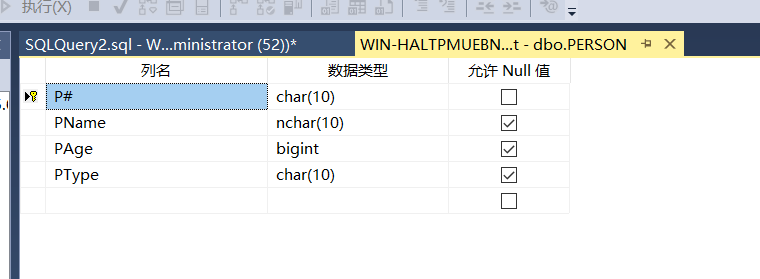
\includegraphics[width=0.3\textwidth]{1.png}
    }
    \subfigure[插入条目]{
        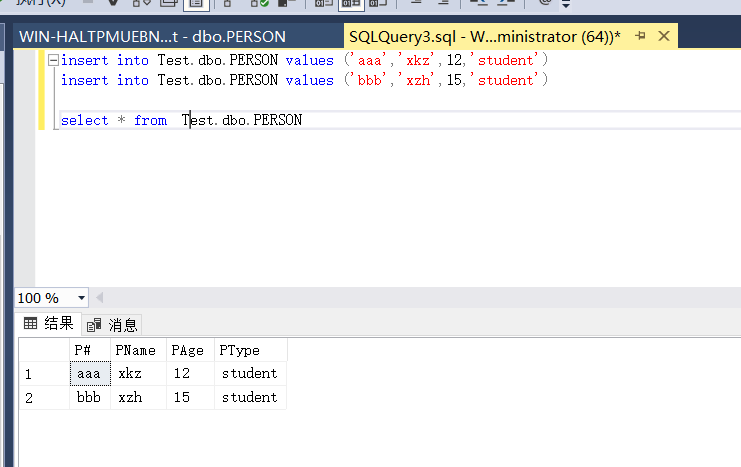
\includegraphics[width=0.3\textwidth]{2.png}
    }
    \subfigure[删除数据]{
        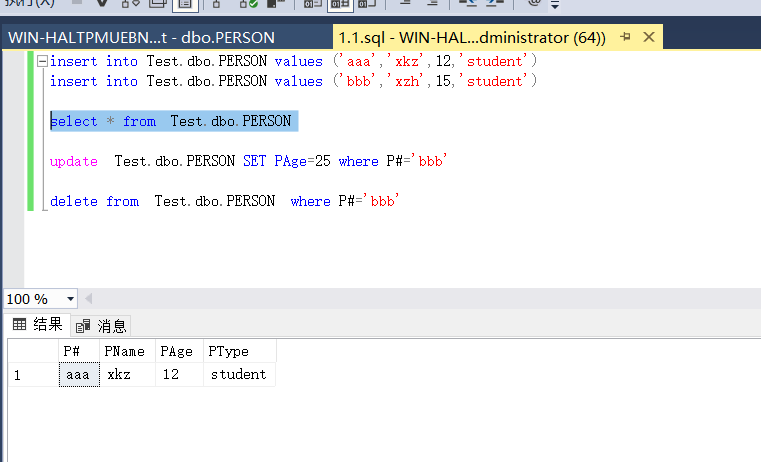
\includegraphics[width=0.3\textwidth]{3.png}
    }
\end{figure}

此外,SMSS也可以一键备份和还原数据库。如图~\ref{fig:backup}
是创建备份的界面。
之后使用如图~\ref{fig:drop}所示的命令删除表,之后仍可以用备份恢复。
\begin{figure}[htbp]
    \centering
    \caption{备份和还原}
    \label{fig:backup}
    \subfigure[备份]{
        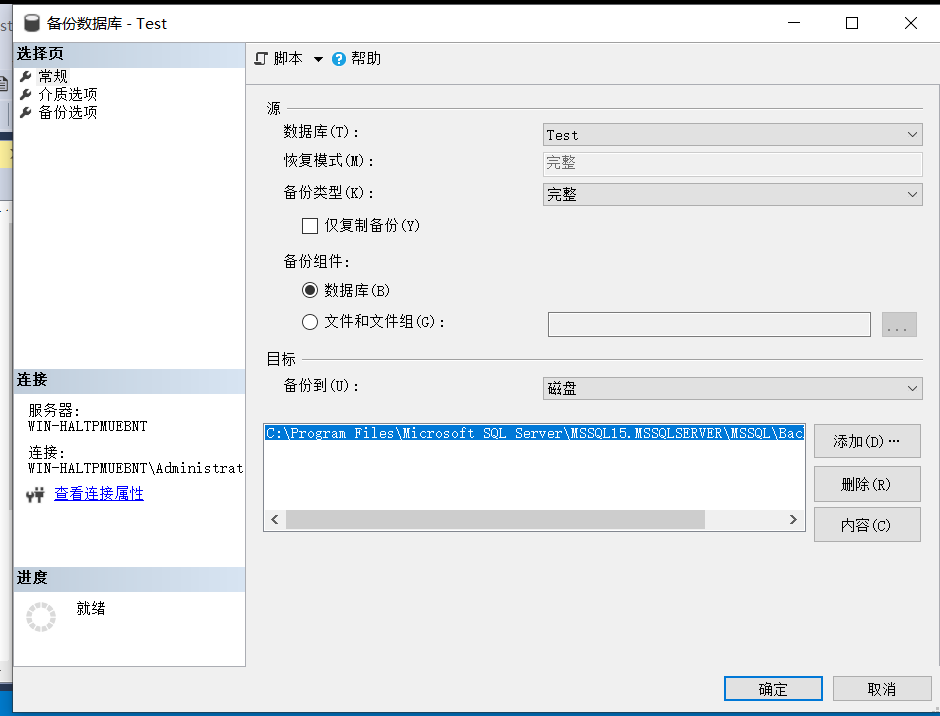
\includegraphics[width=0.4\textwidth]{backup.png}
    }
    \subfigure[删除表]{
        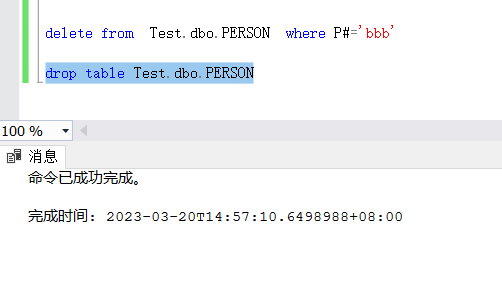
\includegraphics[width=0.4\textwidth]{drop.png}
    }
\end{figure}

需要注意的是,直接还原数据库可能报错:
\begin{quotation}
\textbf{数据库正在使用,无法获得对数据库的独占访问权}
\end{quotation}
这是由于查询时连接了数据库导致的,因此,系统无法还原数据库。因为还原数据库
需要对相应的文件进行写入。

为了解决这一问题,需要在恢复数据库的选项页面勾选“关闭到数据库的现有连接”。
如图~\ref{fig:recovery}。这样就能正常恢复了。
\begin{figure}[htbp]
    \centering
    \caption{还原}
    \label{fig:recovery}
    \subfigure[勾选选项]{
        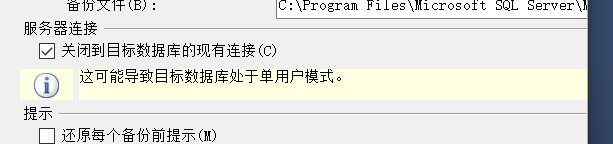
\includegraphics[width=0.4\textwidth]{set.png}
    }
    \subfigure[恢复数据库]{
        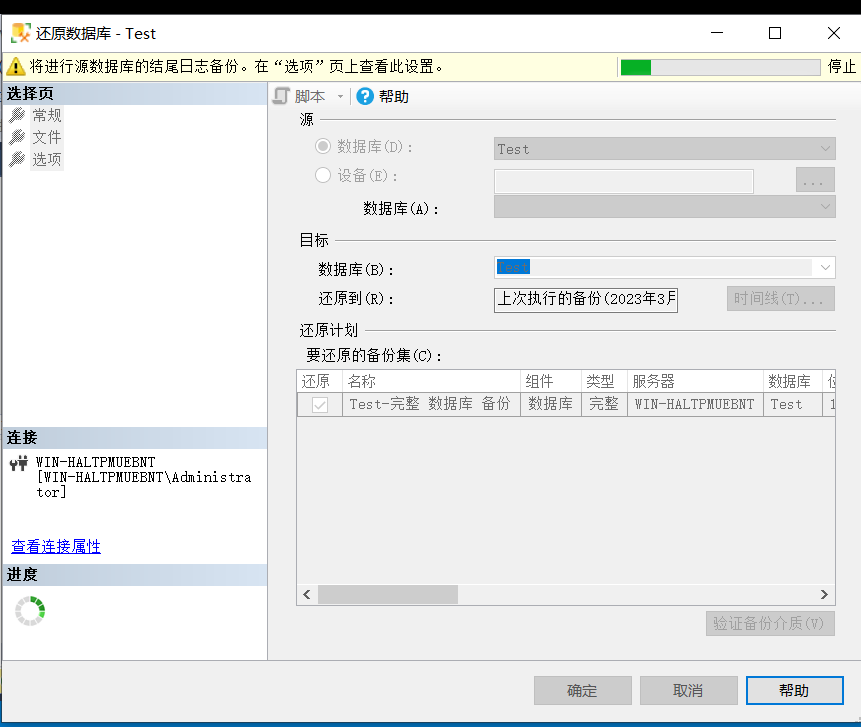
\includegraphics[width=0.4\textwidth]{rec.png}
    }
\end{figure}


\clearpage

\section{实验1.2 数据定义}

\subsection{实验内容}

\begin{enumerate}
    \item 使用CREATE语句创建基本表。
    \item 更改基本表的定义,增加列,删除列,修改列的数据类型。
    \item 创建表的升降序索引。
    \item 取消表、表的索引或表的约束。
\end{enumerate}

\subsection{实验结果}

实验1.2使用SQL语句来管理数据库。首先创建表,执行的语句如图~\ref{fig:sqlcreate}。
\begin{figure}[htbp]
    \centering
    \caption{创建表}
    \label{fig:sqlcreate}
    \subfigure[创建表]{
        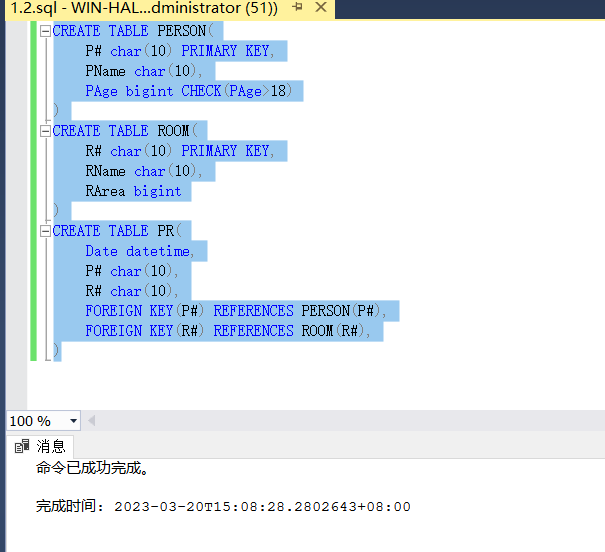
\includegraphics[width=0.3\textwidth]{create.png}
    }
    \subfigure[PERSON表]{
        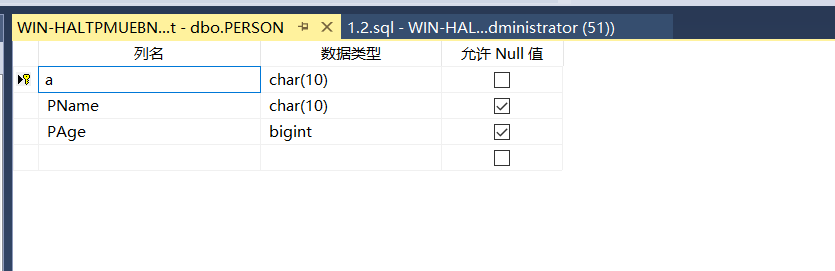
\includegraphics[width=0.4\textwidth]{person.png}
    }
\end{figure}
执行完后可以用SMSS检查PERSON表的结构,可以发现它是正确的。

可以用ALTER语句来修改表的结构,如图~\ref{fig:sqlalter}所示。为PERSON和ROOM
表添加了新的列。
\begin{figure}[htbp]
    \centering
    \caption{修改表}
    \label{fig:sqlalter}
    \subfigure[PERSON表]{
        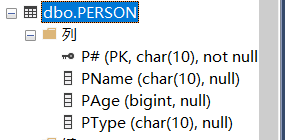
\includegraphics[width=0.4\textwidth]{ptype.png}
    }
    \subfigure[ROOM表]{
        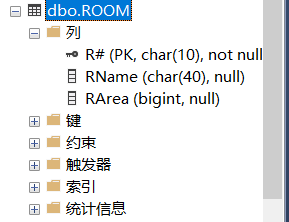
\includegraphics[width=0.4\textwidth]{rarea.png}
    }
\end{figure}
再用ALTER语句和DROP子句,可以删掉RAREA列。如图~\ref{fig:delcol}
\begin{figure}[htbp]
    \centering
    \caption{删除列}
    \label{fig:delcol}
    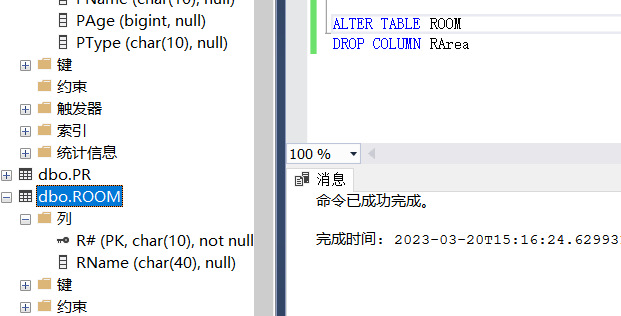
\includegraphics[width=0.6\textwidth]{dropcolumn.png}
\end{figure}
同样地,也可以删除约束PAge的条件,但删除约束要找到约束的ID,然后就可以删除。ID可以在表的约束
一栏中进行查找。如图~\ref{fig:delcons}
\begin{figure}[htbp]
    \centering
    \caption{删除约束}
    \label{fig:delcons}
    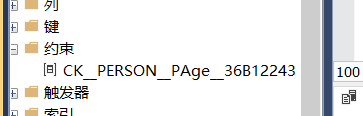
\includegraphics[width=0.6\textwidth]{cons.png}
\end{figure}

为了删除PR中的外键,首先要找到外键的标识ID。和找约束ID一样,在约束一栏中找到外键的ID,然后删除,
如图~\ref{fig:delfkey}所示。再刷新,可以发现约束消失了
\begin{figure}[htbp]
    \centering
    \caption{删除外键}
    \label{fig:delfkey}
    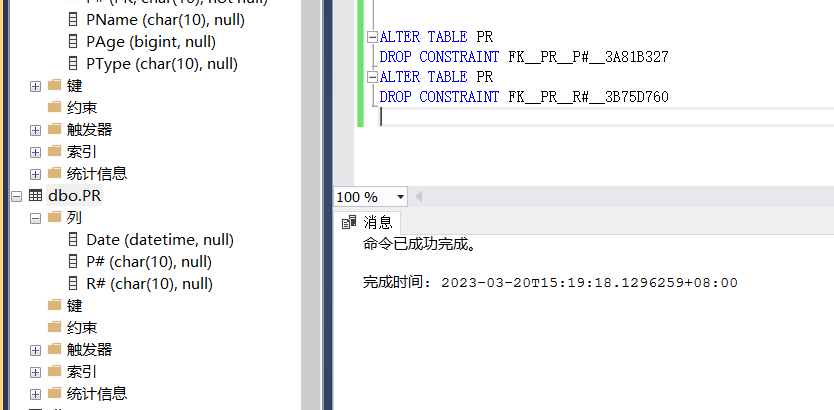
\includegraphics[width=0.6\textwidth]{fkey.png}
\end{figure}

\clearpage

为了创建索引,可以使用CREATE INDEX语句,升序为ASC,降序为DESC,唯一性索引
需要使用UNIQUE关键字。结果如图~\ref{fig:sqlindex}所示。
\begin{figure}[htbp]
    \centering
    \caption{索引}
    \label{fig:sqlindex}
    \subfigure[创建按R\#降序排列的索引]{
        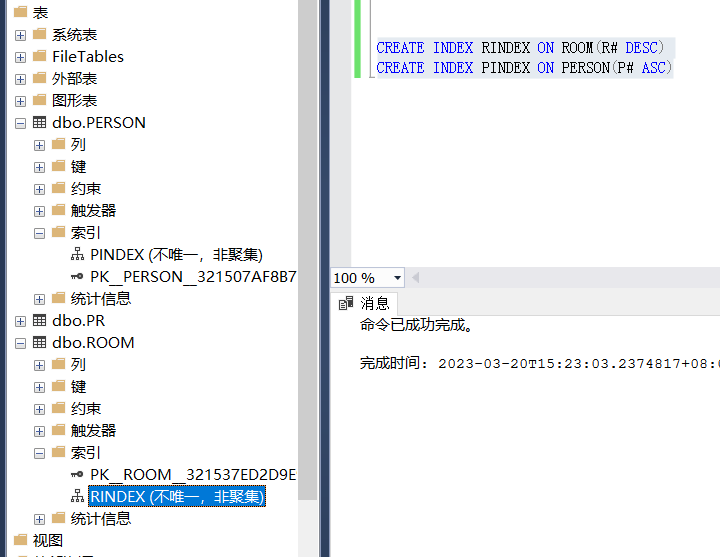
\includegraphics[width=0.3\textwidth]{rindex.png}
    }
    \subfigure[创建按P\#升序排列的索引。]{
        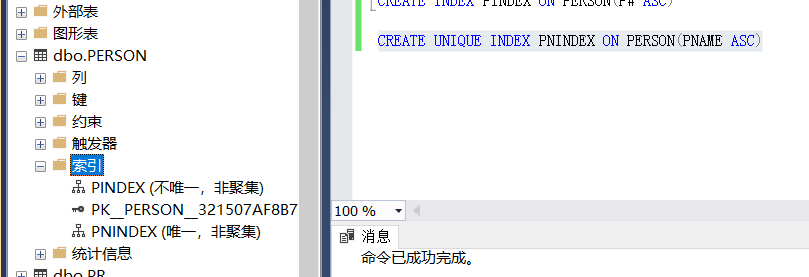
\includegraphics[width=0.3\textwidth]{pindex.png}
    }
    \subfigure[创建表PERSON的按Pname升序排列的唯一性索引]{
        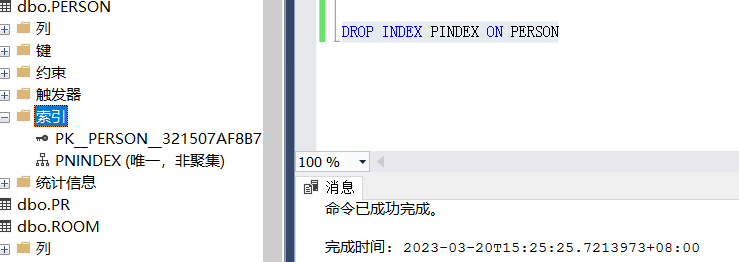
\includegraphics[width=0.3\textwidth]{pnindex.png}
    }
\end{figure}

同样地,删除索引需要使用DROP INDEX语句。如图~\ref{fig:dropindex}所示。
该语句取消表PERSON的P\#升序索引。
\begin{figure}[htbp]
    \centering
    \caption{删除索引}
    \label{fig:dropindex}
    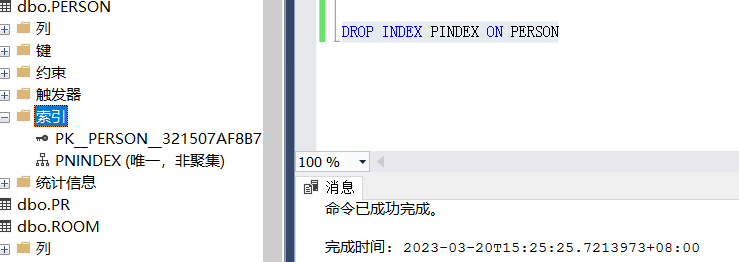
\includegraphics[width=0.6\textwidth]{dropindex.png}
\end{figure}

\clearpage

\section{实验总结}

本次实验中,我分别使用图形用户界面和SQL语句进行了数据库的基本操作,学习了
SQL Server的基本用法,并初步了解了如何解决使用过程中出现的问题。

\appendix

\clearpage

\section{完整代码}

\begin{listing}[H]
	\caption{实验1.2}
	\label{code:full}
    \inputminted{sql}{../code/1.2.sql}
\end{listing}


\end{spacing}

\end{document}